\documentclass{szzclass}
\usepackage{hyperref}

\subject{SAP}
\code{BI-SPOL-28}
\topic{Architektura číslicového počítače, instrukční cyklus počítače,
základní třídy souborů instrukcí (ISA). Paměťový subsystém počítače,
paměťová hierarchie, cache.}

\providecommand{\tightlist}{%
  \setlength{\itemsep}{0pt}\setlength{\parskip}{0pt}}

\begin{document}

\tableofcontents
\newpage
% \hypertarget{spol-28-sap}{%
% \section{SPOL-28-SAP}\label{spol-28-sap}}

% \emph{Architektura číslicového počítače, instrukční cyklus počítače,
% základní třídy souborů instrukcí (ISA). Paměťový subsystém počítače,
% paměťová hierarchie, cache.}
% \newpage
\hypertarget{architektura-ux10duxedslicovuxe9ho-poux10duxedtaux10de}{%
\section{Architektura číslicového
počítače}\label{architektura-ux10duxedslicovuxe9ho-poux10duxedtaux10de}}

\begin{itemize}
\tightlist
\item
  základní části počítače:

  \begin{enumerate}
  \def\labelenumi{\arabic{enumi}.}
  \tightlist
  \item
    Datová část (ALU) - součást procesoru
  \item
    Řídící část (řadič) - součást procesoru
  \item
    Hlavní paměť - často mimo procesor
  \item
    vstupní zařízení
  \item
    výstupní zařízení
  \end{enumerate}
\end{itemize}

\begin{figure}[h]
\centering
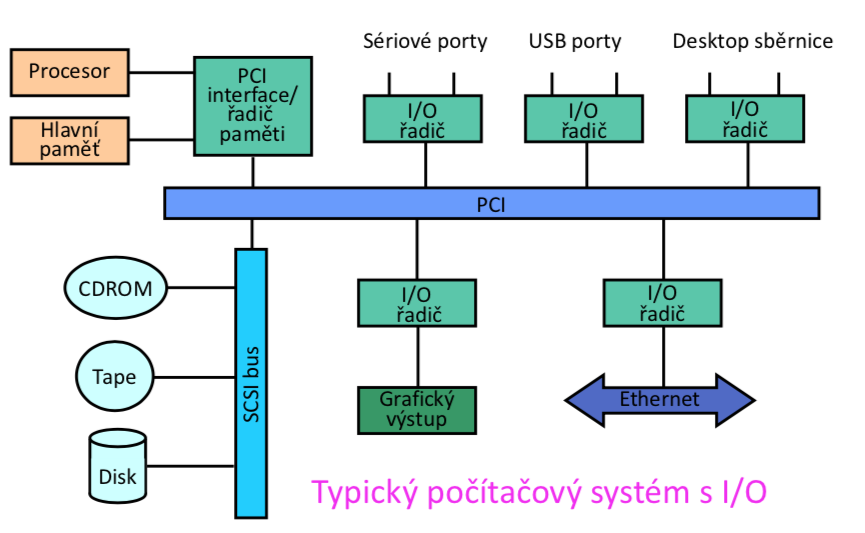
\includegraphics[width=\textwidth]{topics/bi-spol-28/images/hw_architektura.png}
\caption{Harwarová architektura počítače}
\end{figure}

\hypertarget{harward-vs.-von-neuman}{%
\subsection{Harward vs.~Von Neuman}\label{harward-vs.-von-neuman}}

\begin{itemize}
\tightlist
\item
  Harward má oddělenou paměť instrukcí od paměti dat, Von Neuman nikoli
\item
  Harward používaný častěji u malých jednočipových počítačů (ATmega169,\nolinebreak \ldots)
\end{itemize}

\hypertarget{instrukux10dnuxed-cyklus-poux10duxedtaux10de}{%
\section{Instrukční cyklus
počítače}\label{instrukux10dnuxed-cyklus-poux10duxedtaux10de}}

\begin{itemize}
\tightlist
\item
  instrukční cyklus

  \begin{enumerate}
  \def\labelenumi{\arabic{enumi}.}
  \tightlist
  \item
    IF - čtení instrukce (instruction fetch)
  \item
    ID - dekódování instrukce (instruction decode)
  \item
    OF - čtení operandů (operand fetch)
  \item
    IE - provedení instrukce (instruction execute)
  \item
    WE - uložení výsledku (write back)
  \item
    přerušení? (interrupt)
  \end{enumerate}
\item
  nejnižší ``úroveň'' na které může programátor pracovat - staví se
  pomocí ní SW
\item
  \textbf{instrukce} - příkaz zakódovaný jako číslo, musí obsahovat:

  \begin{itemize}
  \tightlist
  \item
    co se má provést (instrukce)
  \item
    s čím se to má provést (operandy)
  \item
    kam uložit výsledek
  \item
    kde pokračovat (např. instrukce \emph{ret} pokračuje jinde než
    \emph{add})
  \end{itemize}
\end{itemize}

\hypertarget{zuxe1kladnuxed-tux159uxeddy-souborux16f-instrukcuxed-isa---instruction-set-architecture}{%
\section{Základní třídy souborů instrukcí (ISA - Instruction Set
Architecture)}\label{zuxe1kladnuxed-tux159uxeddy-souborux16f-instrukcuxed-isa---instruction-set-architecture}}

\begin{itemize}
\tightlist
\item
  zahrnuje:

  \begin{itemize}
  \tightlist
  \item
    typy a formáty instrukcí
  \item
    datové typy, kódování, reprezentace a způsob uložení dat v paměti
  \item
    módy adresování a přístup do paměti dat/instrukcí
  \item
    mimořádné stavy
  \end{itemize}
\item
  umožňuje:

  \begin{itemize}
  \tightlist
  \item
    abstrakci (různé implementace stejné architektury)
  \item
    definici rozhraní mezi SW a HW
  \item
    standardizuje instrukce
  \end{itemize}
\item
  adresace operandů:

  \begin{itemize}
  \tightlist
  \item
    přímá - pracuje se přímo s registrem nebo adresou v operandu
  \item
    nepřímá - v registru/paměti je adresa na data se kterými se pracuje
  \item
    relativní - offset od určíté adresy (v registru nebo immediate)
  \item
    indexovaná - báze + offset

    \begin{itemize}
    \tightlist
    \item
      autoinkrementace/autodekrementace
    \end{itemize}
  \end{itemize}
\end{itemize}

\pagebreak

\hypertarget{stux159adaux10dovuxe1-acumulator}{%
\subsection{Střadačová
(acumulator)}\label{stux159adaux10dovuxe1-acumulator}}

\begin{itemize}
\tightlist
\item
  implicitním operandem ALU je vždy střadač
\item
  byl populární v 50. a 70. letech, protože HW byl drahý a paměti
  rychlejší než CPU
\item
  výhody

  \begin{itemize}
  \tightlist
  \item
    jednoduchý HW
  \item
    minimální stav procesoru =\textgreater{} rychlé přepínání kontextu
  \item
    krátké instrukce (záleží na type daného operátoru)
  \item
    jednoduché dekódování instrukcí
  \end{itemize}
\item
  nevýhody

  \begin{itemize}
  \tightlist
  \item
    častá komunikace s pamětí
  \item
    omezený paralelismus mezi instrukcemi
  \end{itemize}
\end{itemize}

\hypertarget{zuxe1sobnuxedkovuxe1-stack}{%
\subsection{Zásobníková (stack)}\label{zuxe1sobnuxedkovuxe1-stack}}

\begin{itemize}
\tightlist
\item
  využívání ``HW zásobníku'' při vykonávání programu
\item
  např. instrukce ADD vezme 2 nejvyšší hodnoty na zásobníku a do vrchní
  uloží jejich součet
\item
  tento typ byl využit např. u x87 FPU (floating point unit)
\item
  výhody:

  \begin{itemize}
  \tightlist
  \item
    jednoduchá a efektivní adresace operandů
  \item
    krátké instrukce
  \item
    vysoká hustota kódu (tzn. krátké programy)
  \item
    jednoduché dekódování instrukcí
  \item
    snadné napsání překladače (tedy bez optimalizací)
  \end{itemize}
\item
  nevýhody:

  \begin{itemize}
  \tightlist
  \item
    nelze náhodně přistupovat k lokálním datům
  \item
    zásobník je sekvenční (omezuje paralelizmus)
  \item
    těžké omezit přístupy do paměti
  \end{itemize}
\end{itemize}

\pagebreak

\hypertarget{registrovuxe1-gpr---general-purpose-registers}{%
\subsection{Registrová (GPR - General Purpose
Registers)}\label{registrovuxe1-gpr---general-purpose-registers}}

\begin{itemize}
\tightlist
\item
  dnes nejrozšířenější
\item
  RISC a CISC
\item
  výhody:

  \begin{itemize}
  \tightlist
  \item
    registry jsou rychlejší než paměť (dokonce i než cache)
  \item
    lze k nim přistupovat náhodně
  \item
    mohou obsahovat mezivýsledky a lokální proměnné
  \item
    méně častý přístup do paměti =\textgreater{} potenciální možnost
    zrychlení
  \end{itemize}
\item
  nevýhody:

  \begin{itemize}
  \tightlist
  \item
    registrů je omezený počet
  \item
    složitější překladač (např. které hodnoty nechat v registrech\ldots)
  \item
    delší přepínání kontextu
  \item
    registry nemohou obsahovat složitější datové struktury
  \item
    k objektům v registrech nejde přistupovat přes ukazatele
  \end{itemize}
\end{itemize}

\hypertarget{pamux11bux165ovuxfd-subsystuxe9m-poux10duxedtaux10de}{%
\section{Paměťový subsystém
počítače}\label{pamux11bux165ovuxfd-subsystuxe9m-poux10duxedtaux10de}}

\begin{verbatim}
TODO???
\end{verbatim}

\hypertarget{pamux11bux165ovuxe1-hierarchie}{%
\subsection{Paměťová
hierarchie}\label{pamux11bux165ovuxe1-hierarchie}}

\begin{enumerate}
\def\labelenumi{\arabic{enumi}.}
\tightlist
\item
  registry
\item
  caches - extrémně rychlé, drahé, kapacitou menší, umístěné co nejblíž
  k procesoru

  \begin{itemize}
  \tightlist
  \item
    primární cache
  \item
    sekundární cache
  \end{itemize}
\item
  hlavní paměť - rychlé, levnější, větší (např. paměť RAM)
\item
  vnější paměť - pomalé, obrovská kapacita, odkládání (např. pevný disk)
\end{enumerate}

\begin{figure}
\centering
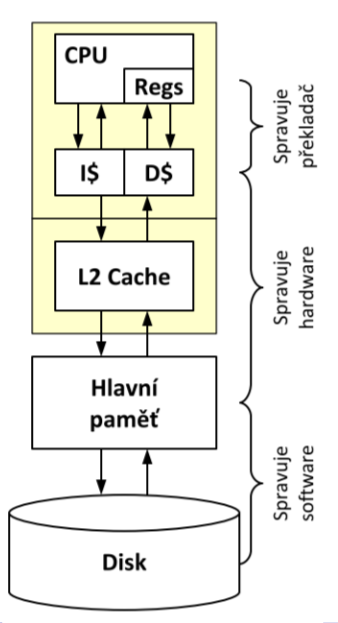
\includegraphics[width=.5\textwidth]{topics/bi-spol-28/images/mem_hierarchie.png}
\caption{Paměťová hierarchie}
\end{figure}

\hypertarget{cache}{%
\subsection{Cache}\label{cache}}

\begin{itemize}
\tightlist
\item
  řeší nízkou rychlost hlavní paměti
\item
  většinou ve více vrstvách (L1, L2, \ldots)
\item
  nižší vrstvy jsou menší rychlejší a dražší
\item
  často jsou využívané asociativní paměti
\item
  čtení:

  \begin{itemize}
  \tightlist
  \item
    \textbf{cache hit} - data jsou v cache nalezena

    \begin{itemize}
    \tightlist
    \item
      \textbf{hit rate} - poměr \emph{cache hit} a počet všech dotazů
    \item
      \textbf{hit time} - doba nalezení údajů v cache a předání
      procesoru
    \end{itemize}
  \item
    \textbf{cache miss} - výpadek cache (je třeba načíst z nižší úrovně)

    \begin{itemize}
    \tightlist
    \item
      \textbf{miss rate} - četnost výpadků cache = 1-hit\_rate
    \item
      \textbf{miss penalty} - doba potřebná k získání z nižší paměti
    \end{itemize}
  \end{itemize}
\item
  zápis:

  \begin{itemize}
  \tightlist
  \item
    pokud není v cache jde rovnou do paměti
  \item
    \textbf{write throught} - nová hodnota se zapíše do cache i do
    hlavní paměti
  \item
    \textbf{write back} - zapíše se do paměti pouze když by měla být z
    cache vyřazena
  \end{itemize}
\item
  více stupňů asociativity - více míst kam uložit paměť se stejným
  klíčem (použití LRU při kolizích pro vyhození)
\end{itemize}

\end{document}